The third prototype built as a proposal of the final TRITIUM detector module was TRITIUM-Aveiro, shown in Figure \ref{fig:TritiumAveiro0},designed and built in the workshop of the University of Aveiro. 

\begin{figure}[h]
\centering
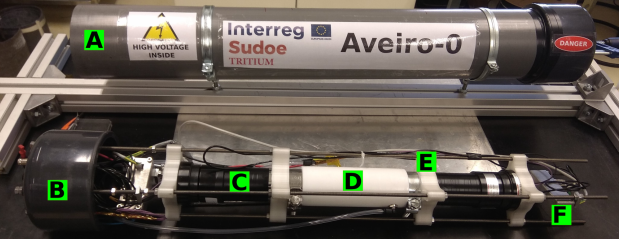
\includegraphics[scale=0.4]{5Prototypes/53FinalPrototypes/531TritiumAveiro/GeneralViewOfAveiroPrototype.png}
\caption{TRITIUM-Aveiro prototype.\label{fig:TritiumAveiro0}}
\end{figure}
This prototype consists of a Teflon vessel (marked as D in Figure \ref{fig:TritiumAveiro0}), shown in Figure \ref{fig:TeflonStructureFibersTritiumAveiro0}, with an internal cylindrical hole of $43~\mm$ diameter and $18~\cm$ length. 

\begin{figure}[h]
\centering
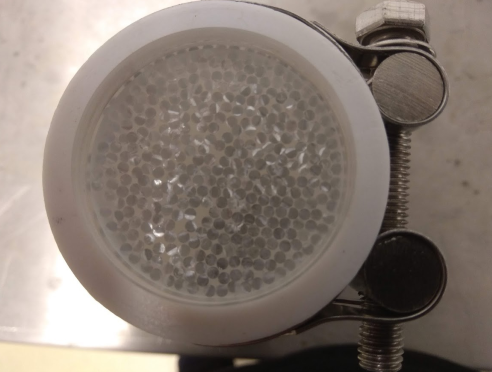
\includegraphics[scale=0.4]{5Prototypes/53FinalPrototypes/531TritiumAveiro/TeflonVessel_Fibers.png}
\caption{Teflon structure and fiber bundle used in TRITIUM-Aveiro prototype.\label{fig:TeflonStructureFibersTritiumAveiro0}}
\end{figure}
This vessel contains $360$ uncladded scintillating fibers of $180~\mm$ length. The fibers are BCF-10 from Saint-Gobain company \cite{DataSheetBCF10Fiber}, which have similar characteristics than the BCF-12 fibers, except the diameter, which is the double, $2~\mm$. A larger diameter is convenient because it facilitates the flow of water around the fibers, reducing problems related to surface tension and ensuring that the entire active volume of the fibers is used for tritium detection. In addition, a large radious increases the rigidity of the fiber. However, this large radious worsens the signal-to-background ratio. The detector active volume for $2~\mm$ fibers is smaller for the same volume, producing a smaller tritium signal and internal volume of the fibers unreachable by tritium decay electrons is larger, producing a larger background. As a result, a lower signal-to-background ratio is obtained. In order to quantify the importance of the fiber diameter, the measurements were compared with similar measurements performed with TRITIUM-IFIC 2 prototype, based on a similar configuration but with $1~\mm$ fibers.

The amount of fibers used in TRITIUM-Aveiro prototype is the maximum which allows the water to flow around the fibers, which are free inside the Teflon vessel. 

These fibers were cleaved with the device developed by TRITIUM but they were neither polished nor cleaned because the automatic polishing machine was not yet developed and it was not feasible to polish 360 fibers by hand. 

The Teflon vessel is totally closed and  a water inlet/outlet were installed in it to allow a constant water flux through it. Two PMMA $10~\mm$ thick windows, located at both ends of the fiber bundle, was used to read the fibers. Two clamps were used to make a tight junction of the Teflon walls and the PMMA. PMMA was chosen for its optical properties, especially its transmission coefficient, which is larger than $95\%$ at the working wavelength. Two PMTs (marked as C in Figure \ref{fig:TritiumAveiro0}) were used to read this prototype in time coincidence. HV was $-1500~\volt$, at which the quantum efficiency is $26\%$. PMTs were attached to both fiber bundle ends by two pieces (marked as E in Figure \ref{fig:TritiumAveiro0}) built with a 3D printer and they were optically coupled to the PMMA windows through optical grease \cite{OpticalGrease}. The PMTs used were R2154-02 2" from Hamamatsu \cite{DataSheetPMTsAveiro}, that have gain and efficiency quite similar to the PMTs used in the other prototypes.

This prototype and its electronics (marked as F in Figure \ref{fig:TritiumAveiro0}), were arranged in a structure, shown in Figure \ref{fig:TritiumAveiro0}, composed of several clamps and four long stainless-steel screws, locked to an external PVC structure, marked as A and B in Figure \ref{fig:TritiumAveiro0}, which protects the prototype from physical damage and provide a light-tight operation environment. This PVC structure is equiped with the necessary feed-through connectors.

Only one prototype was built, which was designed to be installed in the Arrocampo dam and its electronics, based on several PCBs, was specially designed, developed, built and tested to process and analyze the signals of this system, detailed in appendix \ref{App:ElectronicSystemAveiro}. Two interfaces were developed, one to control the PMT power supply, shown in Figure \ref{subfig:GUIHV}, and the other to control the different options of the electronics, such as thresholds and number of counts, shown in Figure \ref{subfig:GUIcounts}.

\begin{figure}
\centering
    \begin{subfigure}[b]{0.65\textwidth}
    \centering
    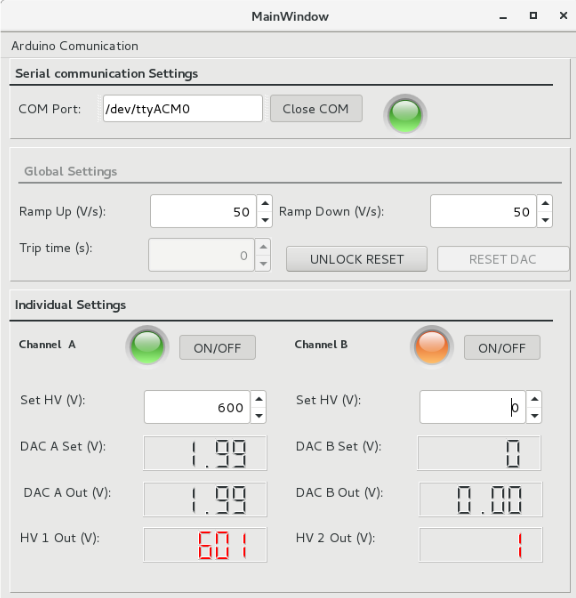
\includegraphics[width=\textwidth]{5Prototypes/53FinalPrototypes/531TritiumAveiro/GUIHVBoard.png}  
    \caption{\label{subfig:GUIHV}}
    \end{subfigure}
    \hfill
    \begin{subfigure}[b]{0.8\textwidth}
    \centering
    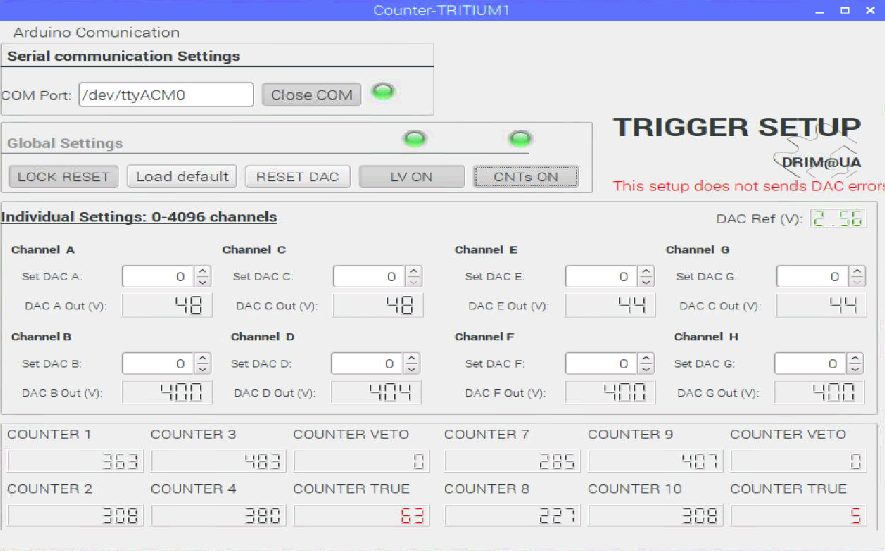
\includegraphics[width=\textwidth]{5Prototypes/53FinalPrototypes/531TritiumAveiro/CounterGUI.png}  
    \caption{\label{subfig:GUIcounts}}
    \end{subfigure}
 \caption{Graphical User Interface developed to control a) PMT HV employed. b) the counter system of the TRITIUM-Aveiro prototype}
 \label{fig:GUITRITIUMAveiro}
\end{figure}

Measurements taken in the laboratories (DRIM and LARUEX laboratories) were used to characterize the detector. For this task, the prototype was firstly filled with pure water, which was used to measure the background of the detector, and next, with a radioactive liquid tritium solution with an activity of $30~\kilo\becquerel/\liter$, which was used to mesure the efficiency and the low detection level of the prototype. The volume of pure water and tritium solution used in TRITIUM-Aveiro prototype was $58~\milli\liter$. 

First, the energy distribution of a single photon of the PMT dark current was measured. To avoid the environmental light detection, the TRITIUM-Aveiro prototype was removed and the measurement was carried out only with the PMTs, the windows of which were covered with black caps. The output signal of the PMTs were digitalized, shaped and pulse-height measured by a CAEN V1724 digitalizer \cite{CAENV1724}. The single-photon energy distribution of both PMTs is shown in Figure \ref{fig:SinglePhotonEnergyDistribution} in which a fit to a Gaussian function was fitted. Due to the electrical noise of the PMT, an extrapolation (dashed line) was needed to be applied.

\begin{figure}[h]
\centering
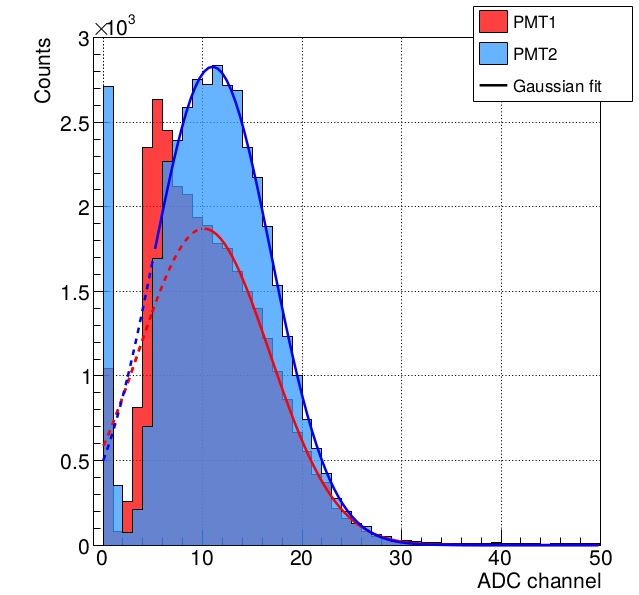
\includegraphics[scale=0.45]{7ExperimentalResultsDetectors/71ExperimentalResultsLaboratory/713TRITIUMAVEIRO0/SinglePhotonEnergyDistribution.png}
\caption{The single-photon energy distribution of both PMTs used in the TRITIUM-Aveiro prototype and their sum \cite{ExperimentalPaperCarlos}.\label{fig:SinglePhotonEnergyDistribution}}
\end{figure}

The distribution obtained with PMT1 deviates from the Gaussian function due to the higher noise in the low energy channels. As DRIM laboratory is not allowed to work with liquid radioactive source such as tritiated water, the first measurements were taken with a $\ce{^{55}Fe}$ radioactive source since the energy of its $\gamma$ emission, $5.9~\keV$, is very close to the energy of tritium electrons. The TRITIUM-Aveiro prototype was coupled to both PMTs using optical grease and, due to its short mean free path in solid materials, the radioactive source was placed inside the Teflon vessel. The prototype was not filled with water for this measurement. The spectra obtained are shown in Figure \ref{fig:55FeMeasurement}. A shift to higher energies is observed in the PMT2 data due to its higher gain and to the closer distance to the radioactive source.

\begin{figure}[h]
\centering
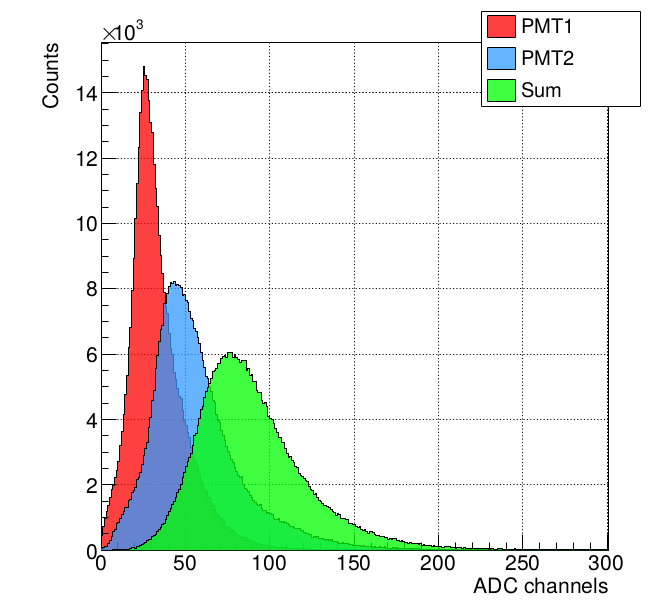
\includegraphics[scale=0.45]{7ExperimentalResultsDetectors/71ExperimentalResultsLaboratory/713TRITIUMAVEIRO0/55FeMeasurement.png}
\caption{Measurement of a $\ce{^{55}Fe}$ radioactive source with the TRITIUM-Aveiro prototype \cite{ExperimentalPaperCarlos}.\label{fig:55FeMeasurement}}
\end{figure}

A measurement with a passive shield was also performed in the DRIM laboratory to quantify the attenuation of the background by lead. The $\ce{^{55}Fe}$ radioactive source was removed and a measurement in counting mode was carried out. This measurements, shown in Figure \ref{fig:LeadShieldTest}, were carried out in three different situations. The first, region A, was performed without shielding, the second, region B, with a lead shield of $2.5~\mm$ thickness and the third, region C, with two lead foil layers. As can be seen, in the region A, the average rate of $2.5$ days is $3.5 \cdot{} 10^3$ counts/min. In the region B, a background supression by a factor of 2 was observed, measuring an average rate of $1.6 \cdot{} 10^3$ counts/min. In the region C, an average rate of $0.9 \cdot{} 10^3$ counts/min was obtained, supressing the background by about a factor of 4.

\begin{figure}[h]
\centering
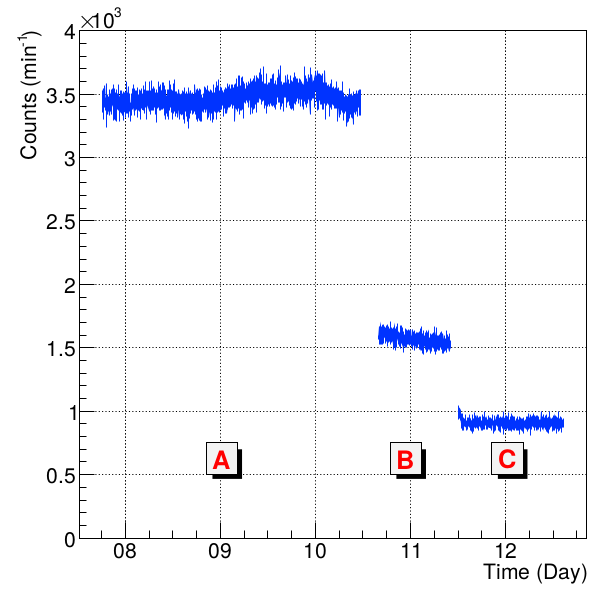
\includegraphics[scale=0.4]{7ExperimentalResultsDetectors/71ExperimentalResultsLaboratory/713TRITIUMAVEIRO0/LeadShieldTest.png}
\caption{Measurement of the background with TRITIUM-Aveiro prototype shielded with different layers of lead, A) without shielding, B) with a lead shield of $2.5~\mm$ thickness and C) with two lead shields of $2.5~\mm$ thickness each one \cite{ExperimentalPaperCarlos}.\label{fig:LeadShieldTest}}
\end{figure}

%It has to be taken into account that the case C is the real situation that is present in Arrocampo since, as it has been shown in section \ref{subsec:SetUpActiveShield}, the thickness of the lead shielding ise $5~\mm$.

To work with a tritiated water, the prototype was installed in the LARUEX laboratory, at the University of Extremadura. 

The background of the prototype was measured during 4 days with the prototype filled with pure water and covered with lead bricks of $5~\cm$ thickness. The time of each measurement is $1$ minut. The data, fitted to a Gaussian function, are shown in Figure \ref{subfig:MeasurementInRealTime}. 

\begin{figure}
\centering
    \begin{subfigure}[b]{0.45\textwidth}
    \centering
    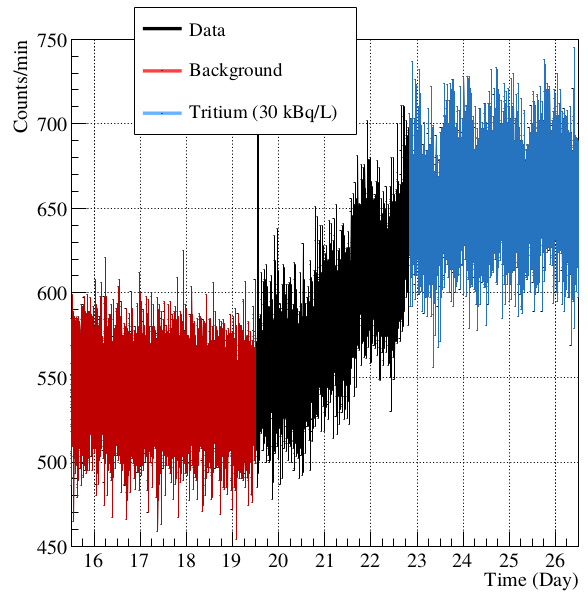
\includegraphics[width=\textwidth]{7ExperimentalResultsDetectors/71ExperimentalResultsLaboratory/713TRITIUMAVEIRO0/Tritium_1min.png}  
    \caption{\label{subfig:MeasurementInRealTime}}
    \end{subfigure}
    \hfill
    \begin{subfigure}[b]{0.45\textwidth}
    \centering
    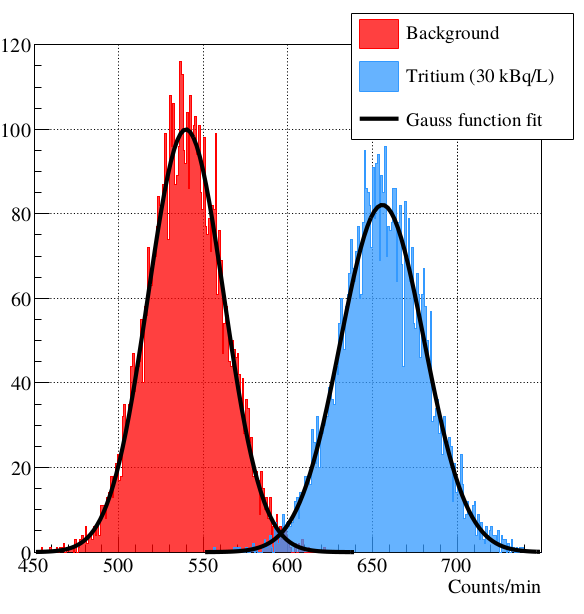
\includegraphics[width=\textwidth]{7ExperimentalResultsDetectors/71ExperimentalResultsLaboratory/713TRITIUMAVEIRO0/Tritium_Gaus_1_min.png}  
    \caption{\label{subfig:DistributionofMeasurement}}
    \end{subfigure}
 \caption{Measurements of the background and tritium liquid source (with an activity of $29.8~\kilo\becquerel/\liter$) performed with the TRITIUM-Aveiro prototype and integred during a minute \cite{ExperimentalPaperCarlos}. a) Counts per minut measured as a function of time. b) Distribution of the acquired data.}
 \label{fig:BackgroundTritium1min}
\end{figure}

An average rate of $540$ counts/min with standard deviation of $22.61$ counts/min was obtained. To calculate the Minimum Detectable Activity (MDA), the detection limit concepts developed by Lloyd A. Currie \cite{CurieLimit} were applied.  The minimum net counts with a probability of a false-negative less than a $5\%$, $N_D$, and minimum net current with the probability of a false-positive less than a $5\%$, $L_C$, called critical level, were calculated by the equations,

\begin{equation}
L_C = 2\kappa\sigma_{Nb} =53 ~\text{counts/min}
\label{eq:EquationCriticalLimit}
\end{equation}
\begin{equation}
N_D = \kappa^2 + 2L_C = 108~\text{counts/min}
\label{eq:EquationNetCounts}
\end{equation}
where $\sigma_{Nb}$ is the standard deviation of the average rate of the background measurements. $L_C$ and $N_D$ refer to the net rate after background subtraction. Therefore, $L_C'$ and $N_D'$, refered to the detector signal (before background subtraction), are $593$ and $648$ counts/min respectively.

To find the MDA, tritiated water was slowly added  so that the tritium water activity increased continuously up to reach the $N_D'$ value. An average of $656 \pm 0.43$ counts/min was obtained, the activity of which was MDA=$29.8~\kilo\becquerel/\liter$, obtained with a Quantulus system.

The tritium detection efficiency was calculated from the ratio of the net tritium rate measured, $1.93 \pm 0.58$ counts/sec, and the activity of the tritium source used. The efficiency obtained is $(6.49 \pm 1.94)\cdot{} 10^{-2}~\liter\second^{-1}\kilo\becquerel^{-1}$.  The specific efficiency is $(1.59 \pm 0.48)\cdot{} 10^{-5}~\liter\second^{-1}\kilo\becquerel^{-1}\cm^{-2}$. Comparing to the specific efficiency obtained with scintillating detectors, Table \ref{tab:PlasticScinTritium}, the specific efficiency of the TRITIUM-Aveiro prototype is close the largest value, obtained by Hofstetter \cite{Hofstetter1, Hofstetter2}. However this prototype has a lower specific efficiency than TRITIUM-IFIC 1. A possible reason is that the fibers used in this prototype are not polished or cleaned. Therefore, the importance of the fiber polishing and cleaning process is again exhibed.

The efficiency uncertainties obtained for this prototype are larger than those obtained in the previous TRITIUM prototypes due to a shorter measurement time, $1$ minute, while that used for the previous prototypes is $10$ minutes. Because of that, longer measurements are studied to quantify the reduction of the MDA of this prototype. The data for an integrated time of $60$ minutes is shown in Figure \ref{fig:Tritium60min}.

\begin{figure}[h]
\centering
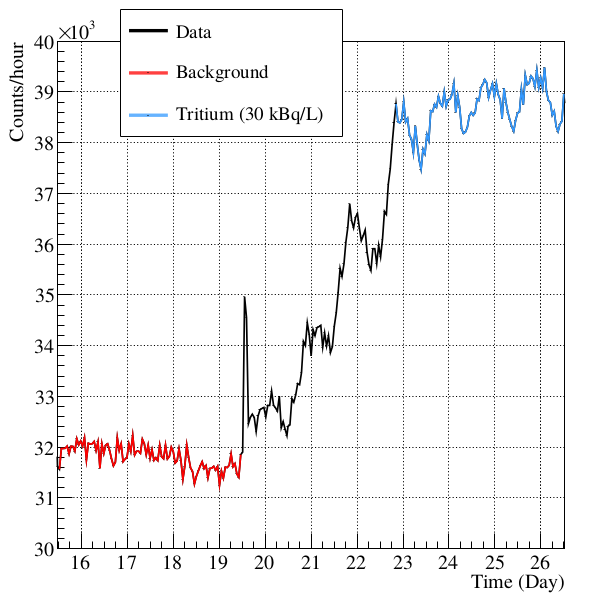
\includegraphics[scale=0.45]{7ExperimentalResultsDetectors/71ExperimentalResultsLaboratory/713TRITIUMAVEIRO0/Tritium_60min.png}
\caption{Measurements of the background and tritium liquid source (with an activity of $29.8~\kilo\becquerel/\liter$) performed with the TRITIUM-Aveiro prototype and integrated during one hour \cite{ExperimentalPaperCarlos}.\label{fig:Tritium60min}}
\end{figure}

The average and uncertainty of the measured background data are $3.186 \cdot{} 10^{4}$ and $228$ counts per hour respectively. The values of $L_C=530$ and $N_D=1043$ counts per hour are obtained respectively from equations \ref{eq:EquationCriticalLimit} and \ref{eq:EquationNetCounts}. Assuming linearity between the measured counts for the background and the tritiated water, the $N_D'$ obtained for this case, $3.872\cdot{}10^4$ counts per hour,  correspons of a MDA of $4.53~\kilo\becquerel/\liter$.

A daily oscilation is clearly observed in the Figure \ref{fig:Tritium60min}, indicating that the measurements are affected by external light. This oscilation begins on the $19^{th}$ day, where the water closed circuit pump was installed, so it is likely that a light leak was introduced in the system.

This prototype was finally installed in the Arrocampo dam to test its functionality and to begin with the tritium level monitoring the measurements of which are reported in section \ref{sec:ResultsArrocampo}.